%%%%%%%%%%%%%%%%%%%%%%%%%%%%%%%%%%%%%%%%%
% baposter Portrait Poster
% LaTeX Template
% Version 1.0 (15/5/13)
%
% Created by:
% Brian Amberg (baposter@brian-amberg.de)
%
% This template has been downloaded from:
% http://www.LaTeXTemplates.com
%
% License:
% CC BY-NC-SA 3.0 (http://creativecommons.org/licenses/by-nc-sa/3.0/)
%
%%%%%%%%%%%%%%%%%%%%%%%%%%%%%%%%%%%%%%%%%

%----------------------------------------------------------------------------------------
%	PACKAGES AND OTHER DOCUMENT CONFIGURATIONS
%----------------------------------------------------------------------------------------

\documentclass[b0paper,portrait]{baposter}
\usepackage{comment}
\usepackage{tikz}
\usepackage{lmodern}
\usepackage[font=small,labelfont=bf]{caption} % Required for specifying captions to tables and figures
\usepackage{booktabs} % Horizontal rules in tables
\usepackage{relsize} % Used for making text smaller in some places
\usepackage{amsfonts}
\usepackage{amsmath, bm}
\usepackage{hyperref}
\usepackage{pgfplots}
\usepackage{graphicx}
%\usepackage{wrapfig}
\usepackage{multicol}
\usepackage{array}
\usepackage{subfig}
\usepackage{url}
\usepackage[export]{adjustbox}
\usetikzlibrary{positioning}
\usetikzlibrary{shapes.geometric}
%\usepgfplotslibrary{patchplots}
%\pgfplotsset{compat=newest}

\graphicspath{{figures/}} % Directory in which figures are stored


\makeatletter
\protected\def\vvv#1{\leavevmode\bgroup\vbox\bgroup\xvvv#1\relax}

\def\xvvv{\afterassignment\xxvvv\let\tmp= }

\def\xxvvv{%
\ifx\tmp\@sptoken\egroup\ \vbox\bgroup\let\next\xvvv
\else\ifx\tmp\relax\egroup\egroup\let\next\relax
\else
%\hbox{\tmp}%original
\hbox to 1.1em{\hfill\tmp\hfill}% centred
\let\next\xvvv\fi\fi
\next}

\makeatother

\definecolor{bordercol}{RGB}{40,40,40} % Border color of content boxes
\definecolor{headercol1}{RGB}{171,205, 239}%{186,215,230} % Background color for the header in the content boxes (left side)
\definecolor{headercol2}{RGB}{192, 192, 192}%{80,80,80} % Background color for the header in the content boxes (right side)
\definecolor{headerfontcol}{RGB}{0,0,0} % Text color for the header text in the content boxes
\definecolor{boxcolor}{RGB}{186,215,230} % Background color for the content in the content boxe
%\definecolor{airforceblue}{rgb}{0.36, 0.54, 0.66}


\definecolor{bluemathlab}{HTML}{065895}
\definecolor{orangemathlab}{HTML}{F79A25}
\newcommand{\highlight}[1]{\textbf{\color{bluemathlab}#1}}
\newcommand{\highlightB}[1]{\textbf{\color{black!15!orangemathlab}#1}}
\newcommand{\rbnics}{\highlightB{\texttt{RB}}\highlight{\texttt{niCS}}}
\newcommand{\fenics}{\texttt{FEniCS}}
\newcommand{\ped}[1]{_{\mathrm{#1}}}
\newcommand{\up}[1]{^{\mathrm{#1}}}
\renewcommand{\r}{\mathbf{r}}
\renewcommand{\d}{\mathrm{d}}
\newcommand{\x}{\times}
\newcommand{\dund}[1]{\underline{\underline{#1}}}
\newcommand{\und}[1]{\underline{#1}}
\newcommand{\mmu}{\boldsymbol\mu}

\def\Put(#1,#2)#3{\leavevmode\makebox(0,0){\put(#1,#2){#3}}}
\usepackage[procnames]{listings}

\definecolor{keywords}{RGB}{255,0,90}
\definecolor{comments}{RGB}{0,0,113}
\definecolor{red}{RGB}{160,0,0}
\definecolor{green}{RGB}{0,150,0}
\definecolor{mygray}{rgb}{0.5,0.5,0.5}

\lstset{language=Python, 
        basicstyle=\ttfamily\small, 
        keywordstyle=\color{keywords},
        commentstyle=\color{comments},
        stringstyle=\color{red},
        showstringspaces=false,
        identifierstyle=\color{green},
        procnamekeys={def,class},
		breaklines=true,
%    	postbreak={\ensuremath{\color{red}\hookrightarrow}},
  numbers=left,                    % where to put the line-numbers; possible values are (none, left, right)
  numbersep=-5pt,                   % how far the line-numbers are from the code
  numberstyle=\tiny\color{mygray}, % the style that is used for the line-numbers
}


\usepackage{algorithm2e}

\SetKwInput{KwIn}{Input}
\SetKwInput{KwOut}{Output}
\newcommand{\forcond}{$i=0$ \KwTo $n$}
\SetKwFunction{FRecurs}{FnRecursive}%
\SetStartEndCondition{ }{}{}%
\SetKwProg{Fn}{def}{\string:}{enddef}
\SetKwFunction{Range}{range}%%
\SetKw{KwTo}{in}\SetKwFor{For}{for}{\string:}{}%
\SetKwIF{If}{ElseIf}{Else}{if}{:}{elif}{else:}{endif}%
\SetKwFor{While}{while}{:}{endwhile}%
\SetKwFor{For}{for}{:}{endfor}%

\renewcommand{\forcond}{$i$ \KwTo\Range{$n$}}
\AlgoDontDisplayBlockMarkers\SetAlgoNoEnd\SetAlgoNoLine%
\SetAlgoLined
\RestyleAlgo{boxruled}
\LinesNumbered

\begin{document}

\background{ % Set the background to an image (background.pdf)
\begin{tikzpicture}[remember picture,overlay]
\draw (current page.north west)+(-2em,2em) node[anchor=north west]
{
\includegraphics[height=1.1\textheight]{background.png}};
\end{tikzpicture}
}

\begin{poster}{
grid=false,
borderColor=bordercol, % Border color of content boxes
headerColorOne=headercol1, % Background color for the header in the content boxes (left side)
headerColorTwo=headercol2, % Background color for the header in the content boxes (right side)
headerFontColor=headerfontcol, % Text color for the header text in the content boxes
boxColorOne= white,%boxcolor, % Background color for the content in the content boxes
%headershape=rounded,%right, % Specify the rounded corner in the content box headers
headerfont=\Large\sf\bf, % Font modifiers for the text in the content box headers
textborder=rectangle,
background=user,
headerborder=closed, % Change to closed for a line under the content box headers
boxshade=plain,
columns=6,
headerheight=0.1\textheight
}
{%
%\hspace{.2cm}
}%{
\includegraphics[height=3.5em]{erc}\hspace{.2cm}\includegraphics[height=7.5em]{aroma-logo}}
%
%----------------------------------------------------------------------------------------
%	TITLE AND AUTHOR NAME
%----------------------------------------------------------------------------------------
%
{\\\vspace{0.25cm} {\huge\bf Constrained Generative Models \\ \vspace{0.25cm} for shape parametrisation}} % Poster title
{\vspace{0.25cm} Guglielmo Padula, Francesco Romor, Giovanni Stabile, Gianluigi Rozza \\ % Author names
{\smaller \vspace{0.25cm} Mathematics Area, mathLab, SISSA, International School of Advanced Studies, Trieste, Italy}
} % Author email addresses
{
} % University/lab logo
\Put(70,2200){
\includegraphics[height=6em]{logo_PyGeM.png}}
\Put(0,2200){
\includegraphics[height=6em]{logo-mathlab_no_borders}}
\Put(665,2200){
\includegraphics[height=6em]{qr}}
\Put(735,2200){
\includegraphics[height=6em]{logo_sissa_cerchio}}

%----------------------------------------------------------------------------------------



\headerbox{Introduction}{name=introduction,below=auto,column=0,row=0,span=6}{
We study  \textbf{generative models} for shape optimization of complex geometries with a large number of parameters; the objective is also to reduce the number of relevant geometrical parameters, for example for modeling naval hulls, and creating new artificial geometries similar to real data, as there are non-generative techniques for creating new real geometries which respect some constraints, for having fixed volume, (see the package PyGem \cite{pygem} developed here at Sissa) but using them can be costly. The real geometries are parametrized by a lesser number of parameters, which in turn increases the performance of reduced order models. 
}



%----------------------------------------------------------------------------------------

%----------------------------------------------------------------------------------------

\begin{posterbox}[name=workflow,below=introduction,span=6,column=0]{Workflow}
\begin{center}
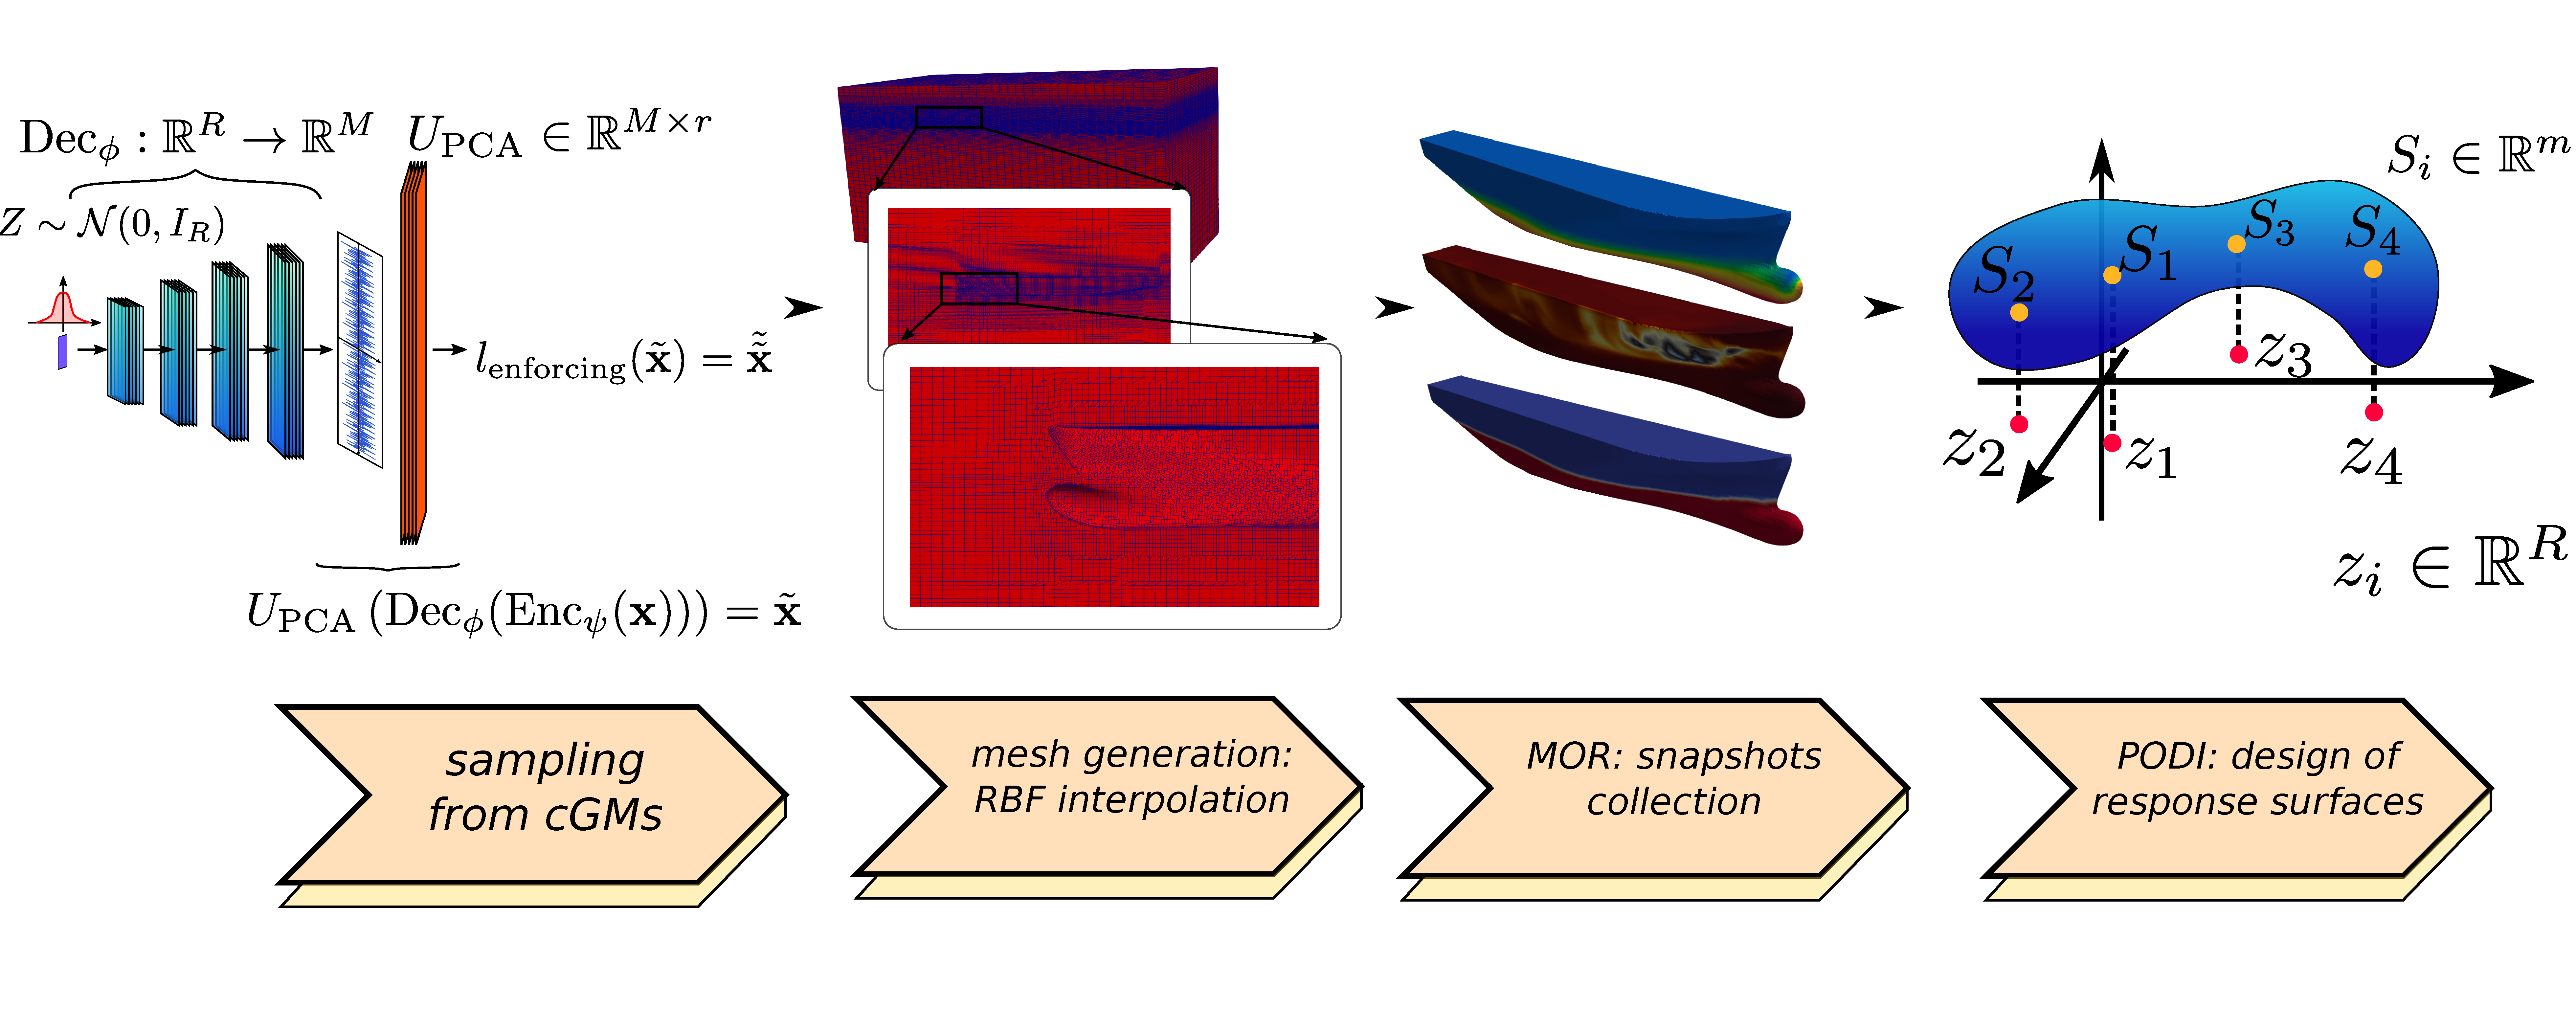
\includegraphics[scale=0.15]{GraphicalAbstract}
\end{center}
\end{posterbox}
\begin{posterbox}[name=vae,below=workflow,span=6,column=0]{Generative models for reduction in parameter space}
Two main model classes:
\begin{itemize}
\item Variational autoencoders(VAE): the figure describes the training using a point cloud mesh of Bulbous bow, and the right figure shows sampling of a deformed Bulbous.\\
\null\\
\begin{tikzpicture}[thick,scale=1, every node/.style={scale=1},
squarednode1/.style={trapezium,draw=blue!60, fill=blue!60, very thick, minimum size=5mm},
squarednode2/.style={trapezium,draw=yellow!60, fill=yellow!60, very thick, minimum size=5mm},
]
\node[inner sep=0pt] (p11) {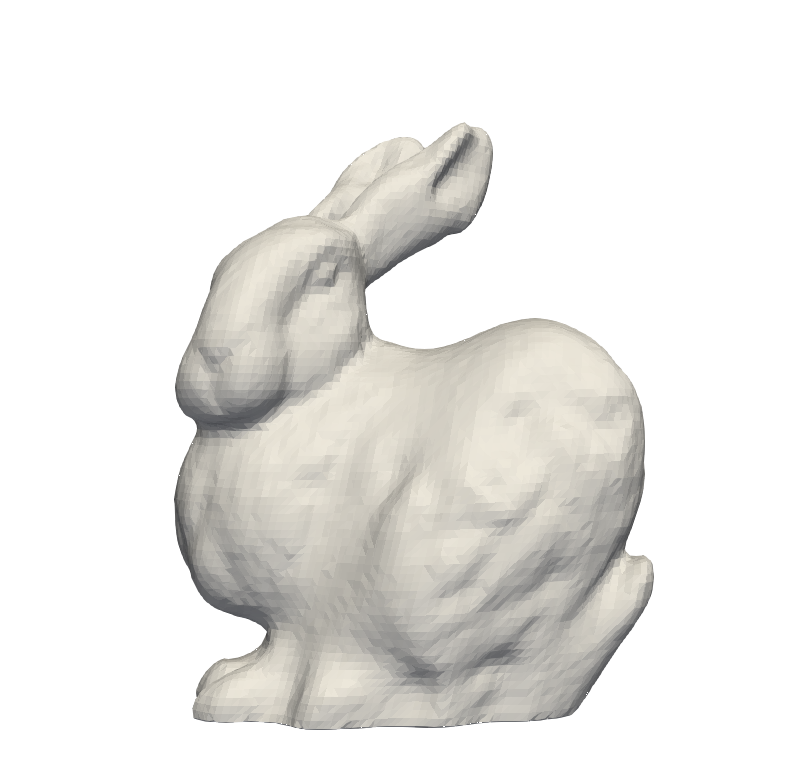
\includegraphics[scale=0.10]{rabbit_0}};
\node[squarednode1, rotate=90,left=of p11,shift={(-1.65,0)}]      (encoder)       [right=of p11]{\textbf{Encoder	}};
\node[inner sep=0pt,shift={(0,-1.65)}] (normal)  [right=of encoder]{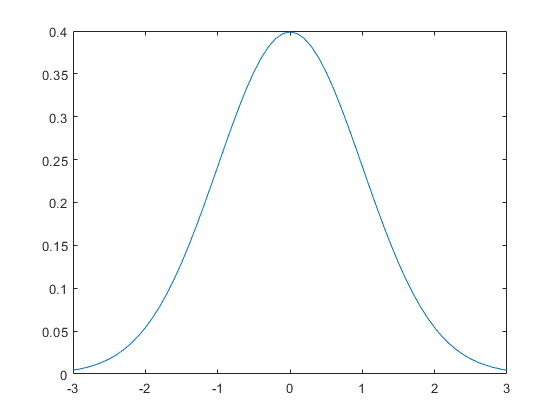
\includegraphics[scale=0.15]{normal}};
\node[squarednode2,rotate=-90,shift={(-1.65,0)}]      (decoder)       [right=of normal]{\textbf{Decoder}};
\node[inner sep=0pt,shift={(0,+1.65)}] (p21) [right=of decoder]{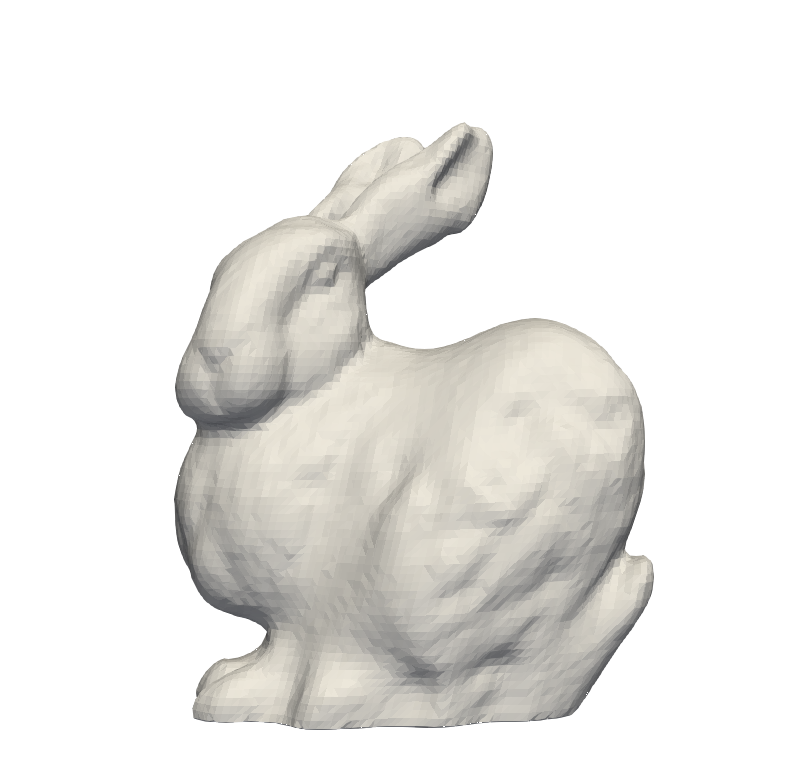
\includegraphics[scale=0.10]{rabbit_0}};

\draw[->] (p11.east) -- (encoder.north);
\draw[->] (encoder.south)-- (normal.west);
\draw[->] (normal.east) -- (decoder.south);
\draw[->] (decoder.north) -- (p21.west);
\end{tikzpicture}\qquad \qquad  \begin{tikzpicture}[thick,scale=1, every node/.style={scale=1},
squarednode2/.style={trapezium,draw=yellow!60, fill=yellow!60, very thick, minimum size=5mm},
]
\node[inner sep=0pt] (normal)  [right=of encoder]{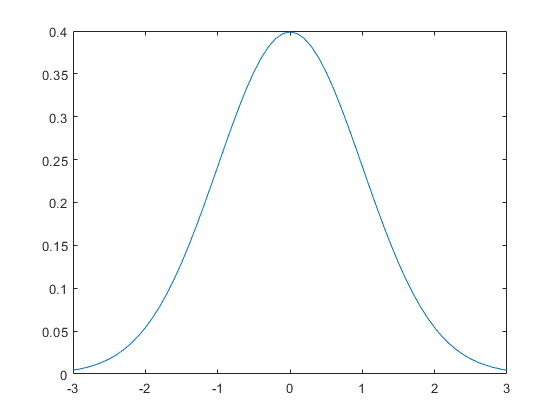
\includegraphics[scale=0.15]{normal}};
\node[squarednode2,rotate=-90,shift={(-1.65,0)}]      (decoder)       [right=of normal]{\textbf{Decoder}};
\node[inner sep=0pt,shift={(0,+1.65)}] (p21) [right=of decoder]{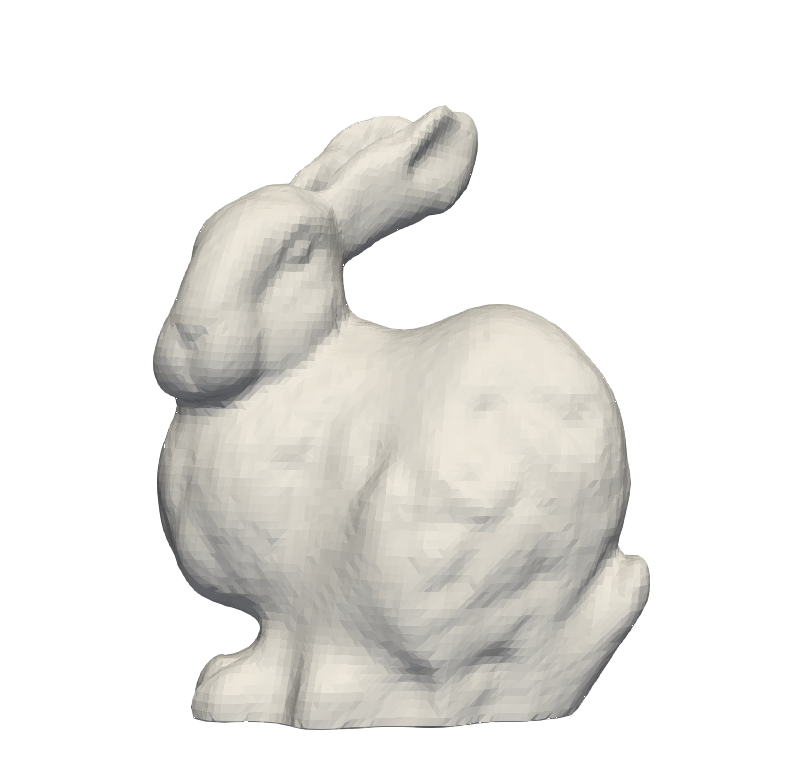
\includegraphics[scale=0.10]{rabbit_1}};

\draw[->] (normal.east) -- (decoder.south);
\draw[->] (decoder.north) -- (p21.west);
\end{tikzpicture}


\item Generative adversarial networks: it is characterized by a generator that samples point cloud mesh of rabbit and by a discriminator that accepts real rabbit (right figure) and rejects deformed ones (left figure).  \\
\null\\
\begin{tikzpicture}[thick,scale=1, every node/.style={scale=1},
bluesquarednode/.style={rectangle, draw=orange!60, fill=orange!60, very thick, minimum size=5mm},
redsquarednode/.style={circle, draw=red!60, fill=red!60, very thick, minimum size=5mm},]


\node[inner sep=0pt] (normal) {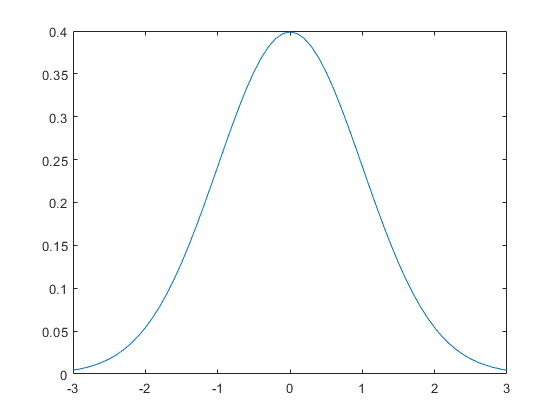
\includegraphics[scale=0.15]{normal}};
\node[bluesquarednode,rotate=-90,shift={(-0.9,0)}]      (generator)       [right=of normal]{\textbf{Generator}};
\node[inner sep=0pt,shift={(0,+0.9	)}] (mesh)  [right=of generator]{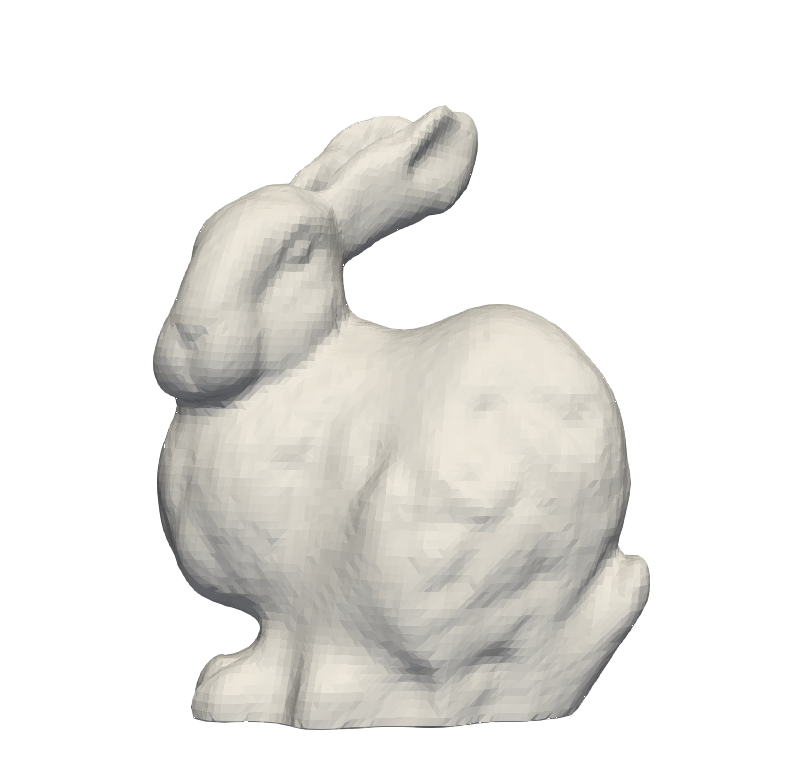
\includegraphics[scale=0.10]{rabbit_1}};
\node[bluesquarednode,rotate=-90,shift={(-1.22,0)}]      (discriminator)       [right=of mesh]{\textbf{Discriminator}};
\node[redsquarednode,shift={(0,1.22)}]      (false)       [right=of discriminator]{FALSE};

\draw[->] (normal.east) -- (generator.south);
\draw[->] (generator.north) -- (mesh.west);
\draw[->] (mesh.east) -- (discriminator.south);
\draw[->] (discriminator.north) -- (false.west);
\end{tikzpicture}\qquad \qquad\ \qquad    \quad \begin{tikzpicture}[thick,scale=1, every node/.style={scale=1},
bluesquarednode/.style={rectangle, draw=orange!60, fill=orange!60, very thick, minimum size=5mm},
greensquarednode/.style={circle, draw=green!60, fill=green!60, very thick, minimum size=5mm},]


\node[inner sep=0pt] (cad)  {
\includegraphics[scale=0.10]{cad}};
\node[inner sep=0pt] (mesh)  [right=of cad]{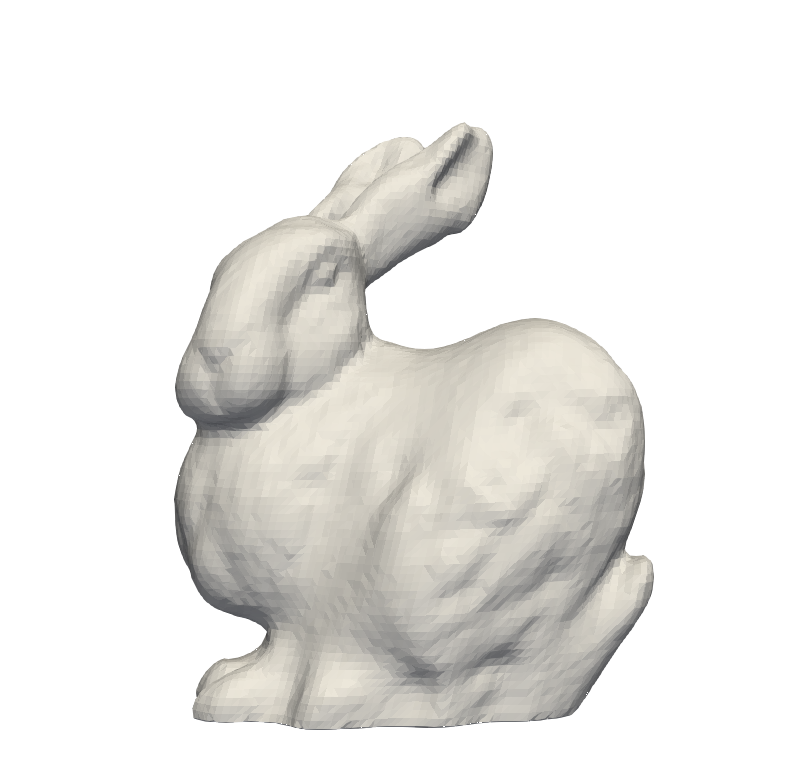
\includegraphics[scale=0.10]{rabbit_0}};
\node[bluesquarednode,rotate=-90,shift={(-1.22,0)}]      (discriminator)       [right=of mesh]{\textbf{Discriminator}};
\node[greensquarednode,shift={(0,1.22)}]      (false)       [right=of discriminator]{TRUE};

\draw[->] (cad.east) -- (mesh.west);
\draw[->] (mesh.east) -- (discriminator.south);
\draw[->] (discriminator.north) -- (false.west);
\end{tikzpicture} \\
\null \\
\null\\
The loss for the discriminator is $ 
 \mathcal{L}_{\mathrm{D}}^{\mathrm{GAN}}=-\mathbb{E}_{x \sim p_{d}}[\log (D(x))]-\mathbb{E}_{\hat{x} \sim p_{g}}[\log (1-D(\hat{x}))]$ and the one for the generator is $\mathcal{L}_{\mathrm{G}}^{\mathrm{GAN}}=\mathbb{E}_{\hat{x} \sim p_{g}}[\log (1-D(\hat{x}))]$.
\end{itemize}
\end{posterbox}

\begin{posterbox}[name=results,below=vae,span=6,column=0]{Results and future work}
We study two test case: one of them is a multifluid Interfoam simulation on the DTCHull, with the bulb deformed using Constrained Free Form Deformation with fixed volume (figure on the left).
As generative models we adopt Variational Autoencoders, Adversarial Autoencoders, Classic Autoencoders and Boundary Equilibrium Generative Adversarial Networks. We validate our model by checking the distribution (on the center) and the performance of reduced order models on quantity of interest (on the right).\\
\hfill\\
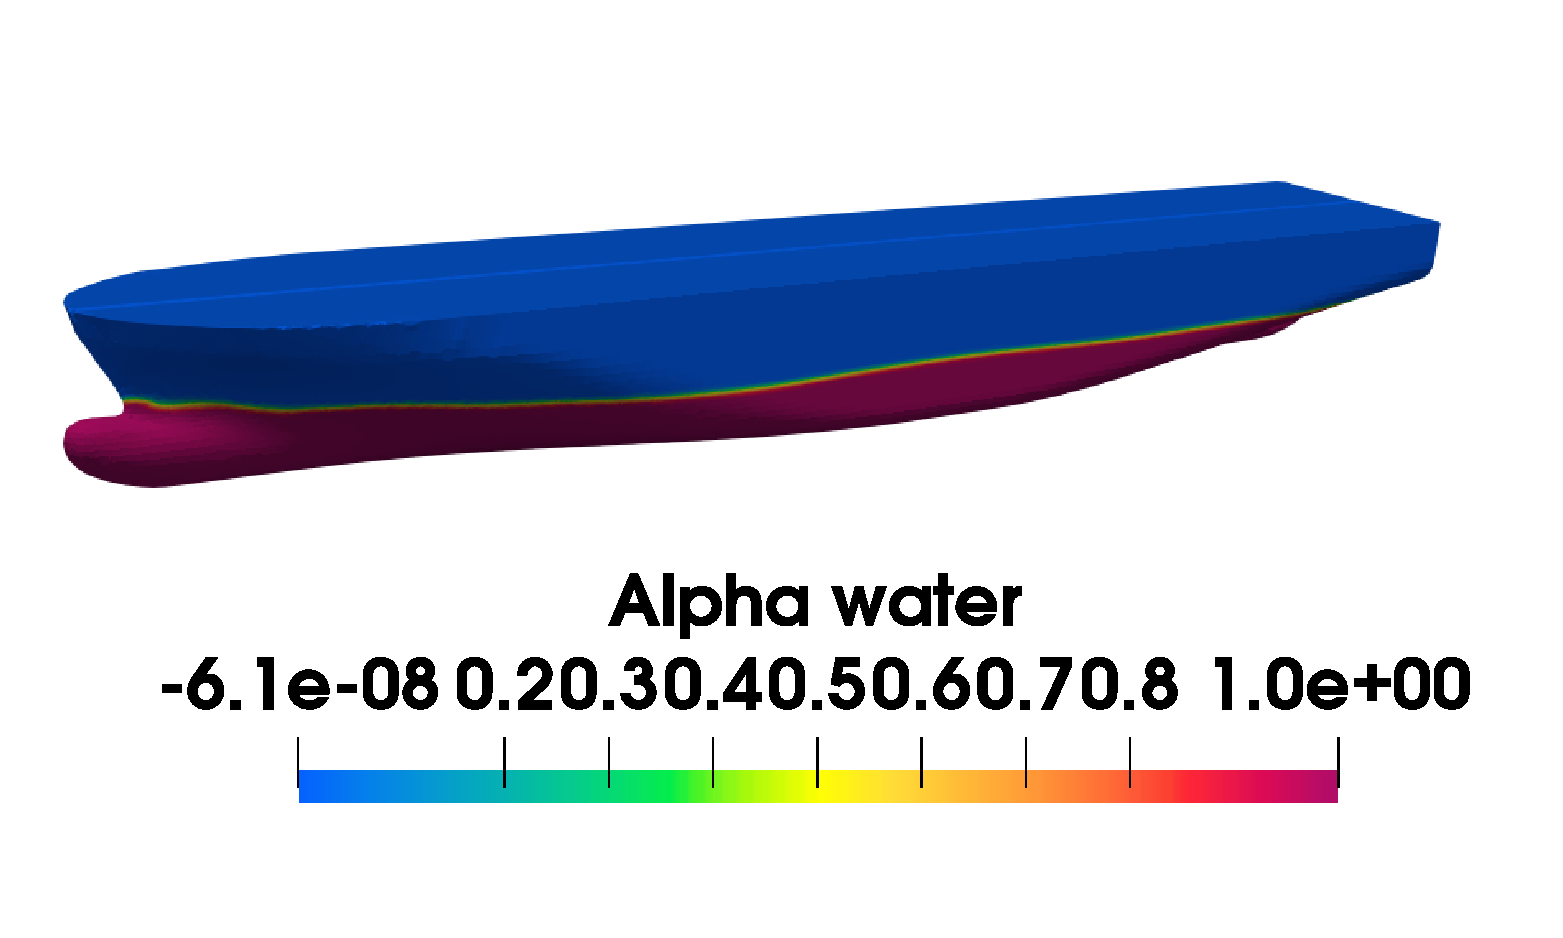
\includegraphics[scale=0.20]{DTCHull_alpha} \quad      \quad     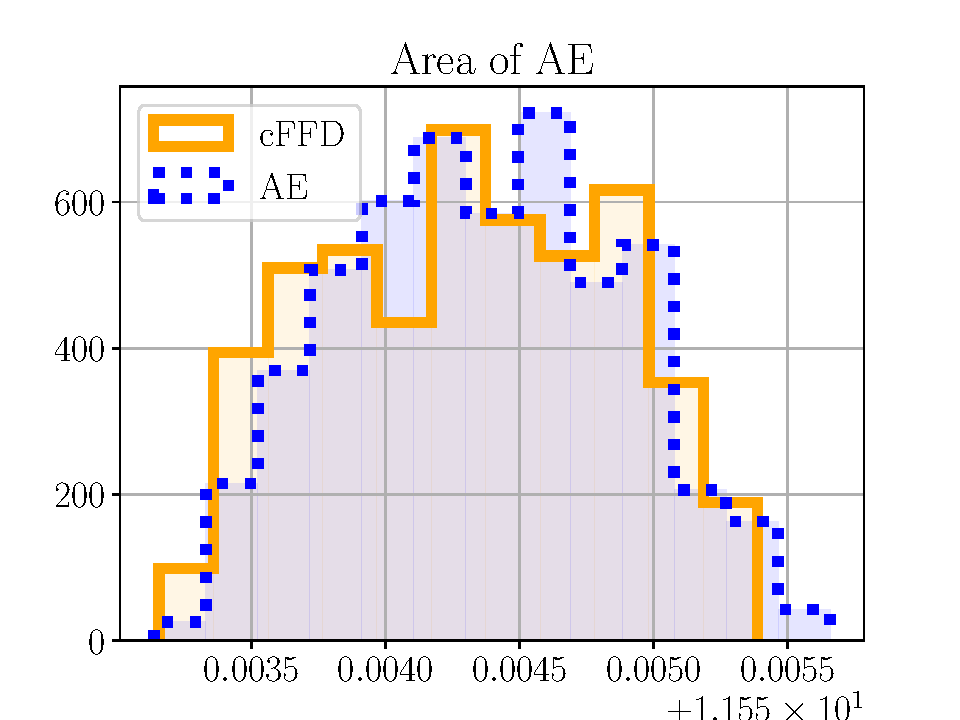
\includegraphics[scale=0.35]{images_Area_hist_AE}   \quad \quad     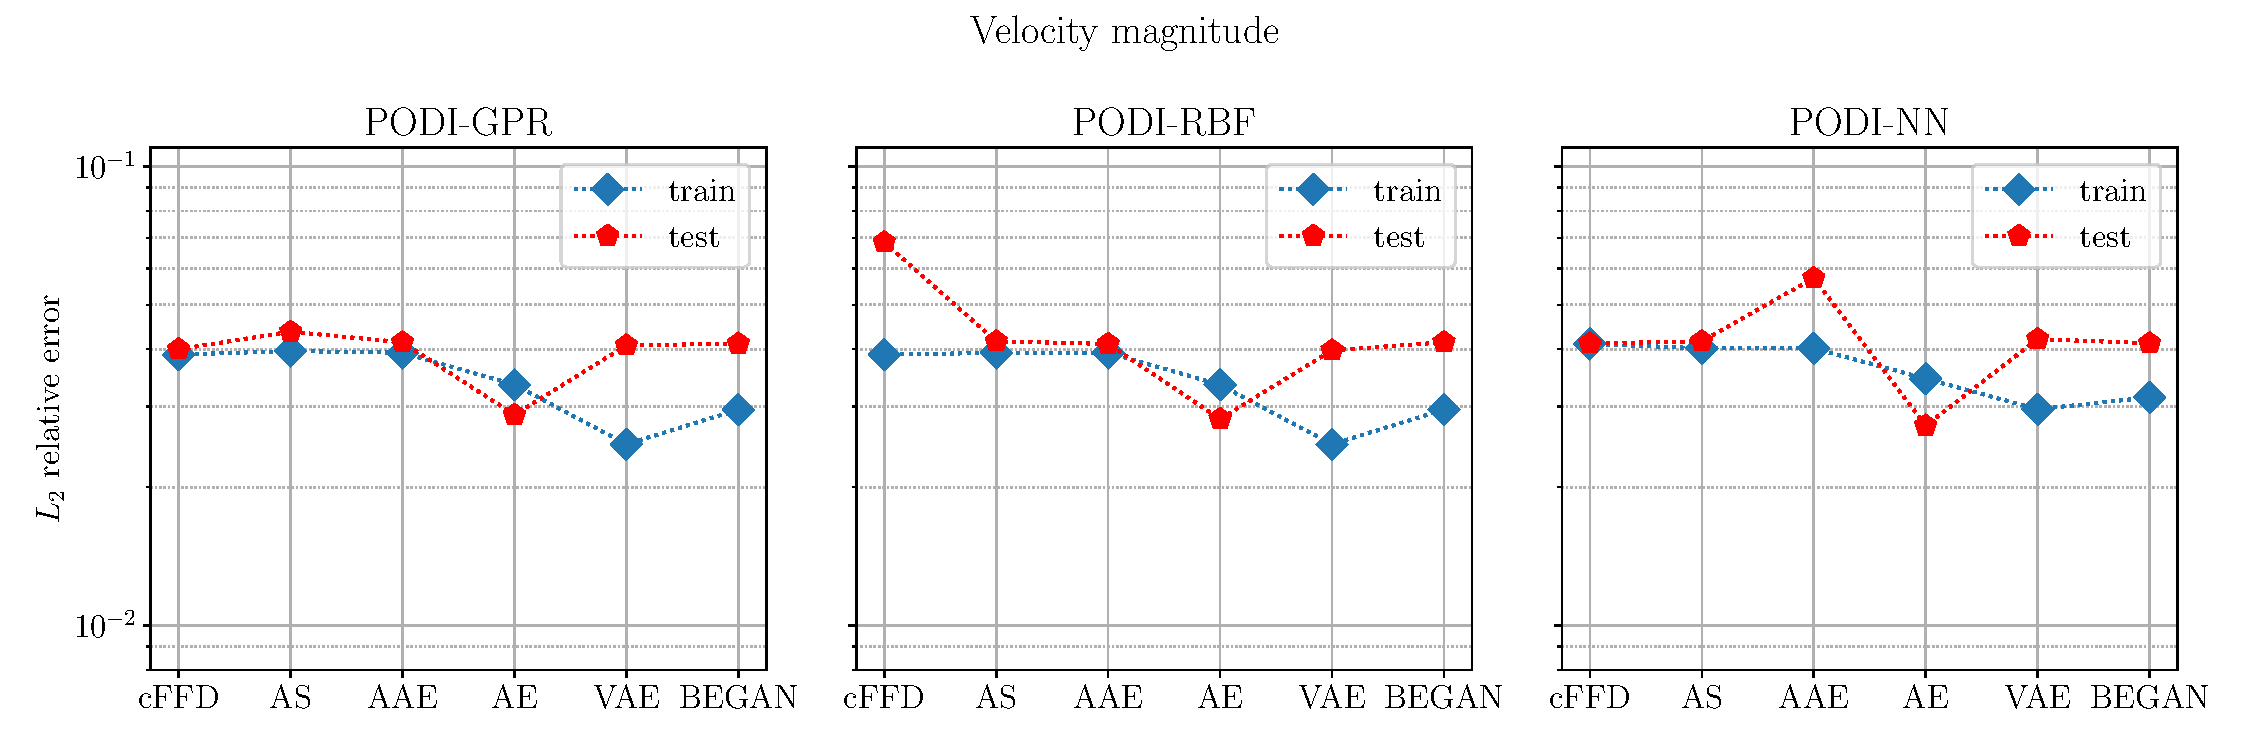
\includegraphics[scale=0.35]{images_DTCHull_u_rom}\\
\hfill\\
The other test case is the deformation of a Stanford Bunny with fixed barycenter. We refer to our paper for the details.\\
As future work, we could try to improve our generative models with the adoption of Graph Neural Networks.
\end{posterbox}
\begin{posterbox}[name=bibliography,below=results,span=6,column=0]{Bibliography and Software References}
%\begin{thebibliography}{9}
%\bibitem{geogram} Geogram, \url{http://alice.loria.fr/software/geogram/doc/html/index.html}
%\bibitem{hello} A numerical algorithm for $L_{2}$ semi-discrete optimal transport in 3D, Bruno Levy, arXiv, 2014
%\bibitem{miao} Variational Autoencoders for Deforming 3D Mesh Models, Qingyang Tan, arXiv, 2018
%\begin{thebibliography}
\begingroup
\renewcommand{\section}[2]{}%
\begin{thebibliography}{9}
 \setlength\itemsep{0.1em}
\small{
\bibitem{pygem}
Pygem, \url{https://github.com/mathLab/PyGeM}
\bibitem{vffd}
 Volume-preserving FFD for programmable graphics hardware.  Hahmann,  S and Bonneau, GP and Barbier,  S and Elber,  G and Hagen,  H, 2011. The Visual Computer.  Springer Science and Business Media LLC.
\bibitem{cffd}
Generative Models for the Deformation of Industrial Shapes with Linear Geometric Constraints: model order and parameter space reductions.  Padula,  G and Romor,  F and Stabile,  G and Rozza,  G., 2023. arXiv:2308.03662.}
\end{thebibliography}
\endgroup
\end{posterbox}

\end{poster}

\end{document}
